\documentclass[10pt,a4paper]{book}
\usepackage{hyperref}
\usepackage{parskip}
\usepackage{listings}
\usepackage{color}
\usepackage{amsmath}
\usepackage{alltt}
\usepackage[pdftex]{graphicx}
\usepackage{graphviz}
\usepackage{multirow}
\usepackage{graphicx}
\usepackage{epstopdf}
\usepackage{geometry}
\geometry{bindingoffset=1cm}

\usepackage{float}
\floatstyle{boxed} 
\restylefloat{figure}

\usepackage[toc]{glossaries}

\begin{document}
\newcommand{\sups}[1]{\ensuremath{^{\textrm{#1}}}}
\newcommand{\subs}[1]{\ensuremath{_{\textrm{#1}}}}
%\newcommand{\lam}[0]{\ensuremath{\textrm{\lambda}}}

\lstset{
  language=caml,
  basicstyle=\scriptsize,
  upquote=true,
  aboveskip={1.5\baselineskip},
  columns=fixed,
  showstringspaces=false,
  extendedchars=true,
  breaklines=true,
  prebreak = \raisebox{0ex}[0ex][0ex]{\ensuremath{\hookleftarrow}},
  frame=single,
  showtabs=false,
  showspaces=false,
  showstringspaces=false,
  identifierstyle=\ttfamily,
  keywordstyle=\color[rgb]{0,0,1},
  commentstyle=\color[rgb]{0.133,0.545,0.133},
  stringstyle=\color[rgb]{0.627,0.126,0.941},
}
\setcounter{tocdepth}{1}
\newglossaryentry{js}
{
  name=JavaScript
  description={is a scripting language used for web applications.}
}

\makeglossaries


  \frontmatter
  \begin{titlepage}
  \begin{flushright}
    Henry Hughes
  \end{flushright}
  \vspace{2.0in}
  \begin{center}
    \Huge Functionally Reactive Web Applications
  \end{center}
  \vfill
  \begin{center}
    \large Computer Science Tripos
  \end{center}
  \vspace{0.1in}
  \begin{center}
    \large Jesus College
  \end{center}
  \vspace{0.1in}
  \begin{center}
    \large 2011
  \end{center}
\end{titlepage}

  \chapter{Proforma}
\begin{center}
\begin{tabular}{r l}
Name and College: & Henry Hughes, Jesus College\\
Project Title: & Functionally Reactive Web Applications\\
Examination and Year: & Computer Science Tripos 2011\\
Word Count: & Approx. 9,400 words\\
Project Originator: & Dr A. Madhavapeddy\\
Project Supervisor: & Dr A. Madhavapeddy\\
\end{tabular}
\end{center}

\section*{Original Aims}
The purpose of this project is investigate the usefulness of Functional Reactive Programming (FRP) when designing and implementing web applications. It will focus on just one method of FRP, using a modified version of the OCaml compiler called \emph{ocamljs} and the library \emph{froc} which is used for reactive programming in OCaml. The project will look how at the speed of applications produced using FRP compare to JavaScript implementations. It will also look at how the language properties of OCaml help the developer develop code which will be type safe and produce the correct output. % 94 words

\section*{Work Completed}
The project implemented three applications using \emph{ocamljs} and \emph{froc}. The first was a tool for rendering log files for threaded programs in a visual format. \emph{froc} was used to redraw the user interface elements whenever the state of the application changed. The second rendered a graph of data with two variables which varied over time. As the time viewed changed, \emph{froc} would update the values for the data points and then reposition them. The final application was a heat map of energy usage in a building. \emph{froc} sets the appropriate colour for the rooms as the time value changed. % 95 words


\section*{Project Difficulties}
None.

  \chapter{Declaration of Originality}
I \emph{Henry Hughes} of \emph{Jesus College}, being a candidate for Part II of the Computer Science Tripos, hereby declare that this dissertation and the work described in it are my own work, unaided except as may be specified below, and that the dissertation does not contain material that has already been used to any substantial extent for a comparable purpose.

Signed 

\vspace{0.4in}

Date

  \tableofcontents

  \mainmatter
  \chapter{Introduction}

This chapter introduces the reasons for the project and the goals it sets out to achieve. It looks at the advantages of web applications and some of the issues currently involved in developing them.

\section{Motivation}
Web applications are becoming increasingly popular due to the disadvantages associated with applications installed on the local machine. One such issue is that the software is difficult to upgrade. Another is that it often costs the user a large one-off amount because it is difficult for the vendor to maintain a service contract when they have distributed a copy of the software binary to the user. If these applications are instead hosted from a remote server then the vendor can worry about upgrading and updating the software and can charge a much smaller but regular fee to the user for the service~\cite{bib:road_ahead}.

There is a variety of programming languages which can be used to create desktop applications. Each provides certain advantages so the developer can choose the language which best suits their needs; this could be anything from the run-time guarantees the programming language provides to rapid development and prototyping. It does not make much difference to the user which language is used; all they want to do is run their favourite application. When writing an application for the Web, however, the programmer is forced to use a specific set of tools. These tools come under the umbrella term \emph{AJAX} (Asynchronous JavaScript and XML). AJAX involves writing client-side code in JavaScript and performing asynchronous requests to the server. This provides a more interactive environment than the classical web application model. The classical model uses the server to create the next web page on the fly and then reloads the current page with the new one. This is often less desirable than AJAX because loading the new page causes a break in the user's work flow~\cite{bib:ajax}.

While JavaScript is a full-featured language, there are other programming languages which provide features it does not. It would be nice if those other languages could be used to write web applications without having to provide a new environment to run them in. In that way, the applications could be written in the developers language of choice but then compiled into JavaScript so would run in current web browsers.

The purpose of this project is to explore the usefulness of writing web applications using \emph{functional} and \emph{reactive} programming techniques.

\section{Concepts}

This section gives a brief overview and some examples of some programming concepts which lead to functional reactive programming (FRP).

\subsection{Glossary of Terms}

\textbf{Imperative Programming}: \emph{A programming language which uses a series of statements to manipulate an implicit state}~\cite{bib:prog}.

\textbf{Declarative Programming}: \emph{These languages are designed to have no state and no assignment. Any state has to be passed into functions as parameters}~\cite{bib:prog}.

\subsection{Scripting Languages}
Scripting is a special type of imperative programming. Scripts are commonly used in rapid prototyping and for performing simple tasks and computations. They often use lazy typing and have minimal structure. JavaScript is a scripting language with C-like syntax which has been adopted by web developers as the most prominent way to perform client-side programming in web applications~\cite{bib:crockford}.

\subsection{Functional Programming}
\label{lab:functional}
The functional programming languages are a subset of the declarative programming languages. With functional programming, \emph{functions} are used as the underlying computation model. Some of the key features of functional programming languages include strong static typing, type inference and polymorphism. These guarantee that any program which passes the type inferencer will not have any type errors~\cite{bib:functional_prog}.

\subsection{Reactive Programming}
Reactive programming provides a way to express how data flows through a program. With imperative programming, if the result of a calculation is assigned to a variable, a change to the inputs of that calculation will not alter the value stored. With reactive programming, however, changes to inputs are passed through the program. Thus the values of variables can depend on the values of other variables and inputs and will update accordingly. Reactive programming languages construct a data-flow graph whose nodes are the variables in the program and whose edges are the dependencies for each variable~\cite{bib:functional_react,bib:lowering}. There are several examples of reactive programming languages. One such example is \emph{ESTEREL}, which is used for programming reactive systems in hardware~\cite{bib:esterel}. Another is \emph{flapjax} which is a language for writing reactive web applications in JavaScript~\cite{bib:flapjax}.

Functional reactive programming is a combination of these two concepts, writing reactive programs using a functional programming language. An example of functional reactive programming can be seen \emph{Functional Reactive Animation}~\cite{bib:fran}.

\section{Purpose}
\label{lab:goals}
The goals of this project are to find solutions to the following questions:

\emph{Is compiling JavaScript pages from a functional programming language a good idea? Where is it useful and what are the downsides?}

\emph{Is reactive programming useful in the context of web applications? Is there a particular situation where the gains (in terms of both computation and code production efficiency) are particularly great?}

  \chapter{Preparation}

\section{Starting Point}

\subsection{JavaScript}
JavaScript is used for client-side scripting on web pages. It is run on the local machine inside the browser environment and can access and modify the Document Object Model (\emph{DOM}), the browsers representation of the  objects on the current web page. By manipulating the DOM at run-time, JavaScript can be used to make interactive user interfaces and dynamic pages.

\subsection{OCaml}
Caml (Categorical Abstract Machine Language) is a general purpose language which supports functional, imperative and object-oriented programming styles. It features a powerful type system which uses parametric polymorphism and type inference. This allows methods to be designed without having to explicitly declare the types of parameters or the result so functions can be reused on many different types of inputs. It also has pattern matching which can be used to direct control flow of the program through functions depending on their inputs.\cite{bib:caml}

OCaml (Objective Caml) is a variant of the Caml language. It is an extension of Caml which adds an object-oriented layer and module system. It is designed for use in developing commercial systems and is the most popular Caml derivative.\cite{bib:ocaml}

\subsection{JavaScript vs OCaml}
In some ways JavaScript is very similar to OCaml. In both languages functions are first class objects, they can be assigned to variables, passed as function parameters and invoked. However the typing systems of OCaml and JavaScript are very different. OCaml types start off generic and get more specific each time they are used. In JavaScript variables themselves do not have a type and so can be reassigned to a value of any type. This can lead to programming errors because you are not guaranteed to know the type of your object at any point. Another difference is that OCaml is checked for errors at compile-time where as JavaScript is checked at run-time. If a piece of code is not executed in a test-run you cannot be sure that it will succeed.

\section{Requirements Analysis}
A successful implementation of this project should:
\begin{itemize}
\item Provide two or more significantly different web applications.
\item These applications must be cross-browser compatible.
\item Each must make use of ocamljs and froc.
\item ...
\end{itemize}

\section{Tools}

\subsection{ocamljs}
ocamljs is a modified version of the OCaml compiler. It uses the standard OCaml compiler up to the point when lambda code is generated, it replaces the last stage where bytecode is generated and outputs JavaScript instead. Figure \ref{fig:ocamlc} shows the stages of the OCaml compiler and ocamljs. \cite{bib:oreilly}

\begin{figure}
  \center{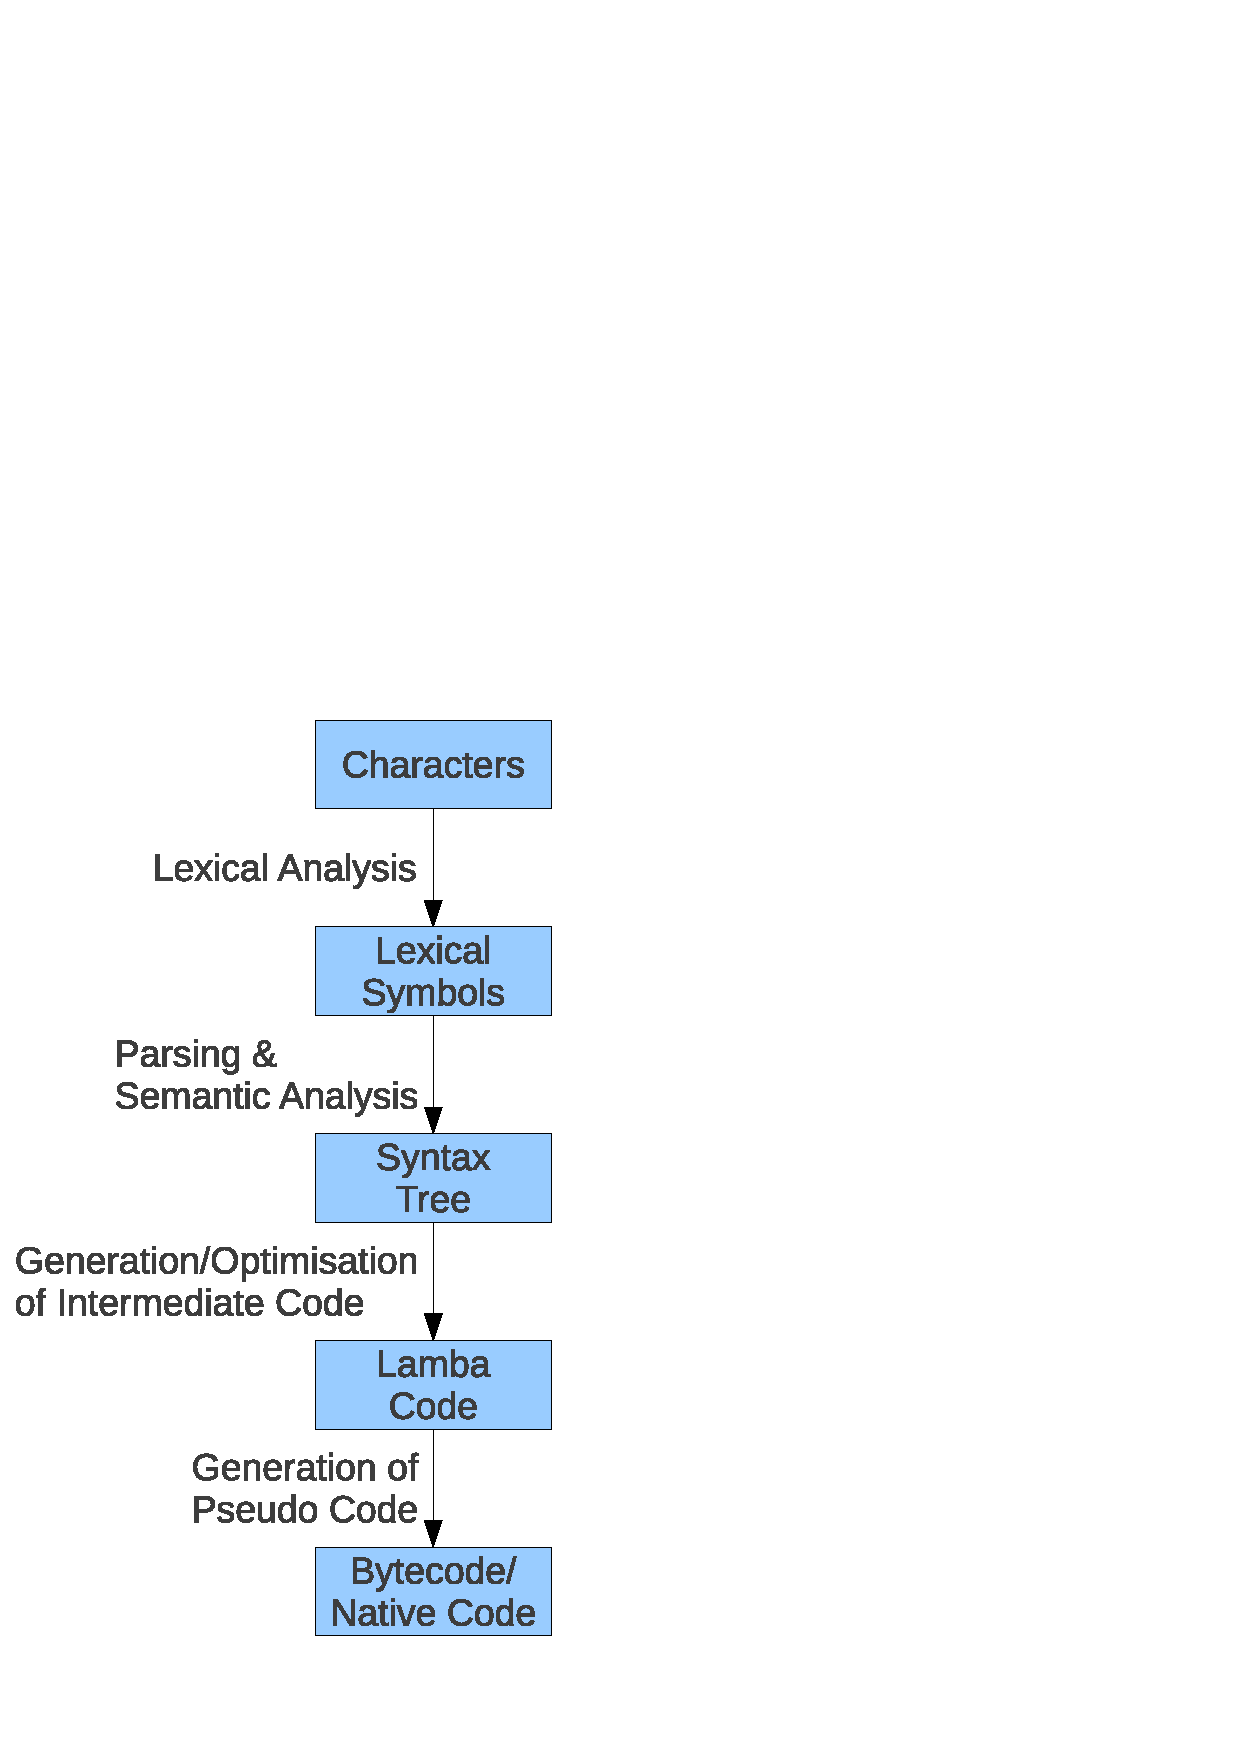
\includegraphics[scale=0.5]{images/ocamlc.pdf}}
  \caption{Stages of the OCaml compiler (ocamlc) and ocamljs.\cite{bib:oreilly}}
  \label{fig:ocamlc}
\end{figure}

\subsubsection{Lambda Code}
Lambda code is based on the $\lambda-calculus$. This notation was invented by Alonso Church in the 1930s. It is used to describe the most basic ways operators and functions can be combined. Conversion from mathematical functions to lambda-expressions is fairly straight forward. Here is a short example:\cite{bib:lambda}

$f(x) = x - 1$ becomes $\lambda.x x-1$

This may not look like a big change but it provides a systematic notation which is good for incorporation into programming. When there are multiple parameters for a function, instead of having a multi-parameter lambda-expression multiple single parameter lambda-expressions are chained. For example:

$\lambda.y \lambda.x x - y$.

Lambda code is very similar to $\lambda-calculus$. Consider the following OCaml program:

\begin{alltt}
let f a b = a+b
let three = f 1 2;;
\end{alltt}

The OCaml compiler can output the lambda representation if the \emph{-dlambda} command-line switch is used. This is the lambda output for the above OCaml:

\begin{alltt}
  (setglobal Simple!
  (let (
  f/58 (function a/59 b/60 (+ a/59 b/60))
  three/61 (apply f/58 1 2))
  (makeblock 0 f/58 three/61)))
\end{alltt}

In this lambda code variables have been renamed. The lambda-expression part is \emph{function a/59 b/60 (+ a/59 b/60)} which is equivalent to \texttt{$\lambda a.\lambda b.a+b$}.

\subsubsection{Lambda to JavaScript}
Functions and exceptions map simply into JavaScript. Integers and floats can be represented as a JavaScript \emph{number} and booleans by the JavaScript \emph{bool}. The standard library functions have been reimplemented in a static JavaScript file.\cite{bib:js_comp}

\subsubsection{Function Applications}
Function applications are a bit more tricky. Functions in JavaScript require the correct number of arguments but in OCaml, functions can receive more (\emph{tail calls}) or less arguments (\emph{partial application}). When we have a partial application we want to return a closure and when we have a tail call we want to apply the extra arguments to the result. This is solved using Simon Peyton Jones' \emph{eval-apply} method.\cite{bib:js_comp,bib:krivines_machine}

\subsubsection{Eval-Apply}
With this scheme the caller is responsible for providing the correct number of arguments to a function. If there are not enough a closure has to be created and if there are too many the left over arguments are applied to the result of the function. This is implemented using the \emph{apply} function outlined in Figure \ref{eval-apply}.\cite{bib:krivines_machine}

\begin{figure}
  \begin{alltt}
f a\subs{1} ... a\subs{n} -> apply\subs{n}(f, a\subs{1}, ..., a\subs{n})

apply\subs{n} = \lam f x\subs{1} ... x\subs{n}
  match arity(f) with
    | 1   -> apply\subs{n-1} (f(x\subs{1}), x\subs{2}, ..., x\subs{n})
    | ...
    | n-1 -> apply\subs{1} (f(x\subs{1}, ..., x\subs{n}), x\subs{n})
    | n   -> f(x\subs{1}, ..., x\subs{n})
    | n+1 -> papp\subs{n+1,n}(f, x\subs{1}, ..., x\subs{n})
    | n+2 -> papp\subs{n+2,n}(f, x\subs{1}, ..., x\subs{n})
    | ...

papp\subs{p,q} = \lam f x\subs{1} ... x\subs{q}. (\lam x\subs{q+1} ... x\subs{p}. f(x\subs{1}, ..., x\subs{p}))
  \end{alltt}
  \caption{Eval-apply implementation}
  \label{eval-apply}
\end{figure}

\subsubsection{ocamljs Example}
Consider a simple function which takes two arguments and returns the summation of them and then an application of this function. Figure \ref{example} shows the OCaml code and compiled JavaScript for this example.

\begin{figure}
  \begin{tabular}{| p{4cm} | p{7.3cm} |}
    \hline
    \textbf{OCaml} & \textbf{JavaScript}\\ \hline
    \begin{alltt}
let f a b = a+b
let three = f 1 2;;
    \end{alltt}
    &
    \begin{alltt}
function () \{
  var f\$58 =
    _f(2, function (a\$59, b\$60) \{
      return a\$59 + b\$60;
    \});
  var three\$61 = _(f\$58, [ 1, 2 ]);
  return \$(f\$58, three\$61);
\}
    \end{alltt} \\ \hline
  \end{tabular}
  \caption{OCaml source and JavaScript output example}
  \label{example}
\end{figure}

\subsection{froc}

\emph{froc} is an OCaml library for reactive programming in OCaml.

\subsubsection{Self Adjusting Computation}
froc uses \emph{self adjusting computation} to push updates to input variables through data paths in the program. Self adjusting means that once the variable has been defined, the program will automatically forward changes to dependencies. This is stored by the program as a \emph{dependency graph}.

\subsubsection{Dependency Graphs}
Given a set of variables and another set of variable dependencies (pairs of variable) a directed graph can be created where the variables form the nodes and the dependencies are the edges. This is a dependency graph and it is used by reactive programs to describe data-flow throughout the program.

\subsection{Behaviors and Events}

Reactive programming uses two polymorphic data type, \emph{behaviors} and \emph{events}. Behaviors are values which vary over time. This could be the colour of an object or it's width for example. Events are a series of time ordered values which correspond to real events such as a mouse press.\cite{bib:lambda}

In order to use these time-varying variables froc provides a way to \emph{bind} them to functions. Naturally this function is called \emph{bind} and has the following syntax:

\texttt{bind : 'a behavior -> ('a -> 'b behavior) -> 'b behavior}

This is a function which takes a behavior of type $\alpha$ and a callback function which converts an $\alpha$ to a $\beta behavior$ and returns a new behavior. Binding other behaviors to a variable is how the dependency graph is constructed, whenever the dependent behaviors change the callback function is invoked with the new values. There is also a syntax shortcut for bind, \emph{\textgreater\textgreater=}.

Any value can be converted into a behavior using the \emph{return} function:

\texttt{return : 'a -> 'a behavior}

Sometimes a callback which is a built in function might be required. Rather than wrapping it in a new function and calling \emph{bind} there is another function called \emph{lift} which does this automatically.

\texttt{lift : 'a behavior -> ('a -> 'b) -> 'b behavior}

There are also multiple argument versions of each function in case you wish to depend on more than one behavior at once. Here are the two argument versions of \emph{bind} and \emph{lift}:

\texttt{bind2 : 'a behavior -> 'b behavior -> ('a -> 'b -> 'c behavior) -> 'c behavior}
\texttt{lift2 : 'a behavior -> 'b behavior -> ('a -> 'b -> 'c) -> 'c behavior}

Consider the following piece of OCaml:


\begin{alltt}
let x = return 1
let y = return 2
let z = return 3

let i0 =
    x >>= fun x ->
        y >>= fun y ->
            return (x + y)
let ans =
    i0 >>= fun i0 ->
        z >>= fun z ->
            return (i0 + z)
\end{alltt}

This program constructs a froc behavior which is the summation of three other behaviors. Figure \ref{add_graph} shows the dependency graph that froc holds internally for this program. Figure \ref{if_graph} shows a more complex dependency graph. In this example if we calculated the value of behavior \emph{b} before behavior \emph{a} and exception could be raised. This example does not cause a divide by zero exception. The first thing this tells us things about froc is that it doesn't always execute every statement in dependency tree, if an intermediate behavior is unused froc doesn't waste computation time on it. This is called \emph{lazy evaluation}. The second thing this tells us is that froc evaluates behaviors in a top-down order. It starts with the outputs and works out which behaviors it needs to compute next from there.\cite{bib:froc}

One final thing to mention is that froc will not propagate changes to a behavior if the callback returns the existing value of the behavior. This is useful because it allows us to put cycles in the dependency graph. If froc did not have this property then a cyclic dependency graph would not terminate.

\begin{figure}
  \centering
  \includegraphics[scale=0.5]{graphs/addition.png}
  \caption{Example dependency graph}
  \label{add_graph}
\end{figure}

\begin{figure}
  \centering
  \includegraphics[scale=0.5]{graphs/if.png}
  \caption{Example if-statement dependency graph}
  \label{if_graph}
\end{figure}

\subsection{HTTP Server}
An HTTP server is required to serve up a web page. At first a stock web server, such as \emph{Apache}, seemed like a good idea because it requires minimal setup. This is good for serving static content (such as HTML pages and JavaScript files) but dynamic content (such as time-dependent JSON messages) proves more tricky. In order to deliver interesting JSON data some server code is required. The two options are to use some sort of server side scripting which Apache can execute, although this requires learning a new language such as \emph{PHP} or to find an implementation of an HTTP server in a language this project is already using (such as OCaml) and modify it such that JSON data can be generated at run-time and delivered to the client.

Using an OCaml HTTP server is the more sensible solution because it gives the greatest amount of time and lets me concentrate on writing the JSON generating code rather than getting stuck learning a new syntax. The OCaml web server I shall use is \emph{ocaml-cohttpserver}\footnote{https://github.com/avsm/ocaml-cohttpserver}.

\subsubsection{json-wheel}
json-wheel is a JSON library for OCaml. It provides a way to build JSON expressions from OCaml objects and visa-versa. \cite{bib:json_rfc}

\section{Architecture}

This project will use the a common design architecture called \emph{client-server}. Client-server is normally based on many clients, one server. It is designed such that the amount of processing performed by the server after each request is minimal. The majority of the computation, which is usually involved in rendering the data as elements on a page, is performed by each client. \cite{bib:dist_arch}

\begin{figure}
  \includegraphics[width=\linewidth]{images/client-server.png}
  \caption{Client/Server Architecture}
  \label{fig:client_server}
\end{figure}

\subsection{Log Viewer}
...

\subsection{Graph}
...

\subsection{Heatmap}
...

\section{Infrastructure}

\subsection{Version Control}
Version control is very important for a software project. It involves breaking the project into a number of changesets. Each change consists of differences to files along with a brief description explaining what changes were made. The idea is that the code is in a consistent state before and after each commit. This is often used in conjunction with pushing changesets to a remote server which is regularly backed up. As a consequence if files get corrupted, deleted or changed in such a way that work has been undone they can be reverted to a working copy.

There are many version control systems. Git is the one used for the ocamljs and froc projects. It has the required functionality and there is a free to use service run by \emph{GitHub}\footnote{http://www.github.com} on the condition at your code is publicly viewable and anyone can fork your repository. The github service also provide some social networking features which allow other developers to follow changes to repositories they are interested in. The repository for this project can be found at https://github.com/hhughes/ocaml-frui.

\subsection{Compiling the Project}
The \emph{GNU Make} system will be used to perform compilation of the project. Make uses shell scripts and dependencies to compile just those parts of the project which have changed since it was last compiled. Compilation of this project is likely to be reasonably quick but it is good practice to use Make for when projects become larger. Make is also a commonly used and simple tool. It is likely that those who clone this repository will already be familiar with the tool.

\section{Design Model}
This project will use the evolutionary model of development because it is difficult to get the solution correct the first time. So by using the evolutionary model the project gets broken up into a number of features which are individually designed, implemented then tested. It is sensible to implement the core functionality first to check that the OCaml to JavaScript compilation is working correctly and then add features one at a time.

[diagram of evolutionary model]

\section{Testing}
In order to test the applications written using ocamljs and froc each application shall have to be recreated using handwritten JavaScript. These implementations should provide the same functionality and use as close to the same algorithms as possible. Each version of each application will be tested using dummy input data and the average execution time of the JavaScript in each case will be used as comparison. Each application should also be tested on at least two web browsers which use different JavaScript engines (for example \emph{Google Chrome} uses \emph{V8} and \emph{Mozilla Firefox} uses \emph{SpiderMonkey}). This is because different browsers will optimise different parts of the code. A note should also be made of the estimated number of man-hours invested in both the ocamljs and pure JavaScript implementations to compare the \emph{ease} of writing the code.

Micro-tests (e.g. implementations of simple algorithms such as \emph{quicksort} or \emph{matrix multiplication}) may also be required if testing results from the web applications are not significant.

\section{Gantt Chart}
...


%\section{Web Applications}
%JavaScript is a client-side scripting language supported by the most popular web browsers so web applications have to use it. Developing in JavaScript, as with all scripting languages, is fairly rapid but as the code base grows keeping track of types of variables and what code gets executed when soon becomes unmanageable. It would be nice if JavaScript could provide the same guarantees for the web application as for programs compiled using OCaml.

%% \section{Dependencies}
%% ocamljs \& froc:
%% \begin{itemize}
%% \item ocaml source
%% \item findlib
%% \item ulex
%% \item camlp4-extra
%% \end{itemize}
%% cohttp-server:
%% \begin{itemize}
%% \item lwt
%% \item react
%% \item libev
%% \item cohttp
%% \end{itemize}
%% ocaml-frui:
%% \begin{itemize}
%% \item ocamljs
%% \item froc
%% \item cohttp-server
%% \item json-wheel
%% \end{itemize}

  \chapter{Implementation}

\section{Log Viewer}
\subsection{JSON}
\subsection{froc}

\section{cohttp-server}
\subsection{State Machine}
\subsection{JSON generation}

\section{froc Extension: froc-lists}
\subsection{Motivation}
\subsection{Implementation}
\subsection{Extensions}

\section{Piechart}
\subsection{Canvases}

\section{Word Cloud}

\section{Dataset Grapher}

\section{Heatmap}

  \chapter{Evaluation}

\section{ocamljs vs JavaScript}
\emph{At what point does writing ocamljs become more effective than js?} Probably once there are multiple developers working on the same piece of web application code. JavaScript quickly becomes unmanageable but OCaml uses modules and classes which can all be independent of each other. This makes it a lot more useful for large scale projects. Also because of the strong type checking, programming errors can easily be identified. This is not so easy with large pieces of JavaScript code where they can become lost and take a long time to debug.

However if the application is fairly small (~100 lines of JavaScript) it would almost certainly be quicker and easier to write it straight in JavaScript, ocamljs is very clunky and repetitive for doing things one off such as setting styles and adding text to elements.

\section{Where froc was useful}
\subsection{Log viewer}
Sort of...
\subsection{Pie chart}
No. We had to do just as much work anyway.
\subsection{Word Cloud}
No. We had to do just as much work anyway.
\subsection{Dataset Graph}
Yes. It was very effective at moving the data points around when needed. It does the minimum work necessary.
\subsection{Heat map}
Yes. It only changes the colours when needed. Again doing the minimum work.

  \chapter{Conclusions}
To wrap up the project this chapter will take a look back at the goals set in the introductory chapter. It will also look at what scope there is for further research and the future of \emph{Functionally Reactive Web Applications}.

\section{Project Successes}
\emph{Is compiling JavaScript pages from a functional programming language a good idea? Where is it useful and what are the downsides?}

Whether it is a good idea to use a functional programming language such as \emph{ocamljs} really depends on what is being developed, the size of the project and what constraints there are on the application. This project has shown that, with one exception, the JavaScript compiled from OCaml took longer to perform the same calculations that with plain JavaScript and it took longer to write the code to do this. It is definitely not effective for rapid prototyping since coding in OCaml takes considerably longer than writing JavaScript. The advantage comes when creating a large application where there are lots of parts as the module system in OCaml is very powerful. The type checker ensures that code changes do not accidentally break interfaces between parts, something which is very easy to do and not so easy to track down in JavaScript.

On the other hand we have to remember we are discussing the development of web applications. The advantage here is that most of the time the server hosting the code is controlled by the developer; every time the user accesses the resource they receive a fresh copy of the application. This makes updating very easy so if things aren't quite right first time, the turnaround time for bug fixes can be extremely short.

\emph{Is reactive programming useful in the context of web applications? Is there a particular situation where the gains (in terms of both computation and code production efficiency) are particularly great?}

It turns out that none of the applications in this project really used the full power of \emph{froc}. Where used it simplified the code however it never really gave any computational advantage. A good application of \emph{froc} would make full advantage of the \emph{lazy evaluation} property of the library to reduce the number of unnecessary calculations performed.

\section{Further Research}
There is much more research to be done on the efficiency of \emph{ocamljs}, for example when does it produce code which can be heavily optimised by the JavaScript engine and can the \emph{ocamljs} compiler be modified to do this for the common case? The question as to when \emph{froc} was useful in web application was also left unanswered. It could be investigated whether \emph{froc} is more useful in situations where more user interaction is involved.

\section{What's Next?}
There is already a commercial use for web applications written in higher level languages. Google, for example, have used the \emph{Google Web Developer Toolkit} (GWT) to create their \emph{Google Moderator} and \emph{Google Wave} applications~\cite{bib:gwt}. GWT provides Java libraries and a compiler that produces a JavaScript application from Java source code. Functional programming is also becoming more popular in commercial situations. An example is the \emph{Xen Cloud Platform} management stack (called XAPI) which is written in OCaml~\cite{bib:xapi}. Maybe soon we shall see the functional programming advocates writing web applications too.
 

%  \backmatter
  \clearpage
\addcontentsline{toc}{chapter}{Bibliography}
\begin{thebibliography}{99}

\bibitem{bib:road_ahead}
Paul Graham,
\emph{The Road Ahead}.
\url{http://www.paulgraham.com/road.html}

\bibitem{bib:ajax}
Jesse James Garrett,
\emph{AJAX: A New Approach to Web Applications}.
\url{http://www.robertspahr.com/courses/web1/ajax_web_applications.pdf}

\bibitem{bib:prog}
Doris Appleby,
\emph{Programming Languages: Paradigm and Practice}.
McGraw-Hill Companies Inc,
1997

\bibitem{bib:crockford}
Douglas Crockford,
\emph{A Survey of the JavaScript Programming Language}.
\url{http://www.crockford.com/javascript/survey.html}

\bibitem{bib:functional_prog}
Paul Hudak,
\emph{Conception, evolution, and application of functional programming languages}.

\bibitem{bib:functional_react}
Zhanyong Wan \& Paul Hudak,
\emph{Functional reactive programming from first principles}.

\bibitem{bib:lowering}
Kimberley Burchett, Gregory H. Cooper \& Shriram Krishnamurthi,
\emph{Lowering: a static optimization technique for transparent functional reactivity}.

\bibitem{fundatastructures}
Chris Okasaki,
\emph{Purely Functional Data Structures}.
Cambridge University Press, Cambridge,
1998

\bibitem{bib:caml}
INRIA,
\emph{About Caml}.
\url{http://caml.inria.fr/about/index.en.html}

\bibitem{bib:ocaml}
INRIA,
\emph{Objective Caml}.
\url{http://caml.inria.fr/ocaml/index.en.html}

\bibitem{bib:oreilly}
Emmanuel Chailloux, Pascal Manoury and Bruno Pagano,
\emph{Développement d'applications avec Objective Caml (translation)}.
O'Reilly France

\bibitem{bib:lambda}
J. Roger Hindley and Jonation P. Seldin,
\emph{Lambda-Calculus and Combinators: an Introduction}.
Cambridge University Press,
2008

\bibitem{bib:js_comp}
Jake Donham,
\emph{How ocamljs compile OCaml}.
\url{http://code.google.com/p/ocamljs/wiki/Jscomp}

\bibitem{bib:krivines_machine}
Xavier Leroy,
\emph{From Krivine's Machine to the Caml implementations}.
\url{http://pauillac.inria.fr/~xleroy/talks/zam-kazam05.pdf}

\bibitem{bib:froc}
Jake Donham,
\emph{How froc works}.
\url{http://ambassadortothecomputers.blogspot.com/2010/05/how-froc-works.html}

\bibitem{bib:dist_arch}
George Reese,
\emph{Chapter 7: Distributed Application Architecture, Database Programming with JDBC and Java, Second Edition}.

\bibitem{bib:make}
GNU Operating System,
\emph{Make}.
\url{http://www.gnu.org/software/make/}

\bibitem{bib:json_rfc}
Douglas Crockford,
\emph{RFC4627}.
\url{http://www.ietf.org/rfc/rfc4627.txt}


\end{thebibliography}

  \printglossaries
  \appendix
  \chapter{Code}

\section{OCaml}

\section{JavaScript}


\end{document}
